
\section{Results}

%Results:	control	input,	system	states,	comment	on	the	requirements,	and	comparisons	
%between	CompSOC and	MATLAB	outcomes
Figure \ref{fig:finalresult} shows the comparison of results between Simulink and CompSOC platform on the "optimal results" configuration shown in Table\ref{tab:poles}. While the simulation and experiment match for most parts, the minor deviations can be attributed to the exact delay differences between the platforms as discussed in \ref{sec:stad}. Then in Figure \ref{fig:Sresult} the derived values are displayed.


\begin{figure}[h!]
	\begin{center}
		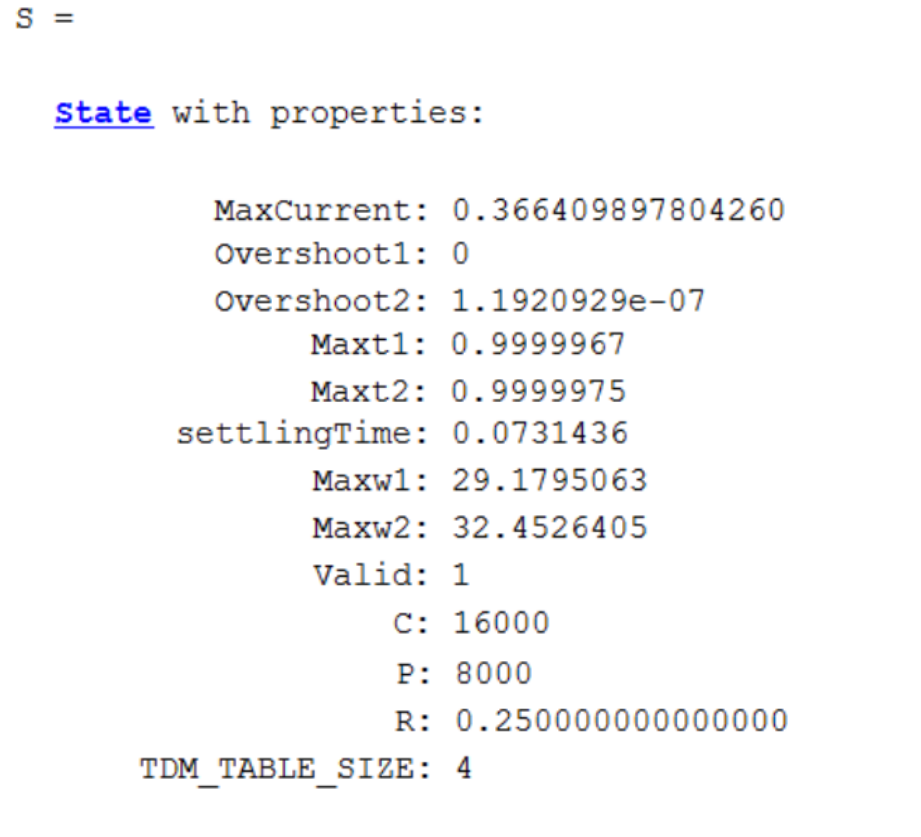
\includegraphics[width=0.5\linewidth]{img/S}
		\caption{Final values for the best solution found. All are well within required design parameters}
		\label{fig:Sresult}
	\end{center}
\end{figure}

\begin{figure}[h]
	\begin{center}
		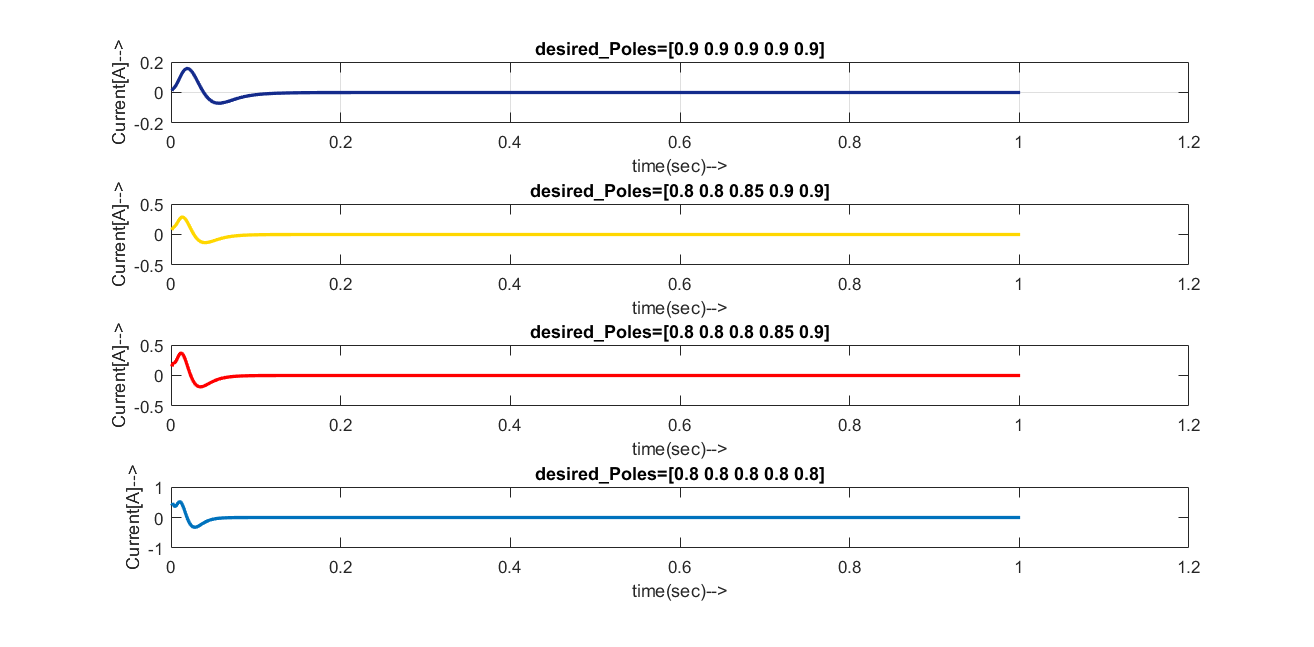
\includegraphics[width=0.8\linewidth]{img/current}
		\caption{The input current for each of the options presented in Figure \ref{fig:qoc2} and Table \ref{tab:poles}}.
		\label{fig:current}
	\end{center}
\end{figure}

